\documentclass[a4paper,12pt]{article}

\usepackage[T2A]{fontenc}
\usepackage[utf8]{inputenc}
\usepackage[russian]{babel}
\usepackage{cmap}

\usepackage{amsmath,amssymb,mathtools}
\usepackage[a4paper,left=25mm,right=15mm,top=20mm,bottom=20mm]{geometry}
\usepackage{indentfirst}
\usepackage{graphicx}
\usepackage{float}
\usepackage{caption}
\usepackage{booktabs}
\usepackage{enumitem}
\usepackage{titlesec}
\usepackage[unicode,hidelinks]{hyperref}

\captionsetup{labelsep=endash,font=small,skip=4pt}
\addto\captionsrussian{\renewcommand{\figurename}{Рисунок}\renewcommand{\tablename}{Таблица}}

\titleformat{\section}{\normalfont\large\bfseries}{\thesection}{0.6em}{}
\titleformat{\subsection}{\normalfont\normalsize\bfseries}{\thesubsection}{0.6em}{}
\titlespacing*{\section}{0pt}{14pt}{6pt}
\titlespacing*{\subsection}{0pt}{10pt}{4pt}

\setlength{\parindent}{1.25cm}
\setlength{\emergencystretch}{1.5em}
\linespread{1.1}
\setlist{itemsep=1pt,topsep=3pt}

\graphicspath{{figures/}}
\newcommand{\code}[1]{\texttt{#1}}

\begin{document}

\begin{center}
  {\Large\bfseries Одномерное уравнение теплопроводности:\\[2pt]
   формула Пуассона и функция Грина\par}
  \vspace{6pt}
  {Отчёт по заданиям А и Б\par}
  \vspace{4pt}
  {Выполнили: Садчев~Р.\,В., Богомолов~С.\,С., Стрельцов~Б.\,С.\par}
\end{center}

\noindent\textbf{А.} Функция, которая находит решение задачи Коши для
одномерного уравнения теплопроводности на прямой по формуле Пуассона или через
функцию Грина и выводит его анимированный график.

\noindent\textbf{Б.} Функция, которая находит решение задачи для уравнения
теплопроводности на полупрямой через функцию Грина и выводит его анимированный
график. Вариант граничного условия: $u_x(0,t)=\mu(t)\cdot\nu(t)$.

Язык~--- Python. Все вычисления выполняют функции, написанные самостоятельно:
сетка, формулы Симпсона (обычная и адаптивная), средних прямоугольников и трапеций
(\code{heatlab/numint.py}), функции Грина (\code{heatlab/kernels.py}) и сборка
решений (\code{heatlab/line.py}, \code{heatlab/halfline.py}). Библиотеки
\code{numpy} и \code{scipy} не используются, готовые решатели и функции
интегрирования~--- тоже. Из стандартной библиотеки взят только модуль
\code{math} (элементарные функции $\exp$, $\sin$, $\sqrt{\ }$), \code{matplotlib}
и \code{tkinter}~--- только для рисования и окна программы.

% ======================================================================
\section{Задание А. Задача Коши на прямой}

\subsection{Постановка задачи}

\begin{equation}\label{eq:A}
  u_t=a^{2}u_{xx}+f(x,t),\quad -\infty<x<\infty,\ t>0;\qquad u(x,0)=\varphi(x).
\end{equation}
Функции $\varphi(x)$, $f(x,t)$, число $a>0$ и длительность $T$ вводит
пользователь; $f\equiv0$~--- однородное уравнение.

\subsection{Метод}

Функция Грина задачи~\eqref{eq:A} (фундаментальное решение)~---
температура от мгновенного единичного источника, помещённого в точку $\xi$ в момент $t=0$:
\begin{equation}\label{eq:K}
  G(x,\xi,t)=\frac{1}{2a\sqrt{\pi t}}\exp\!\left(-\frac{(x-\xi)^2}{4a^2t}\right),\qquad
  \int_{-\infty}^{\infty}G\,d\xi=1,\qquad G\xrightarrow[t\to0]{}\delta(x-\xi).
\end{equation}
Решение~--- суперпозиция таких источников (формула Пуассона) плюс интеграл
Дюамеля для внешнего источника:
\begin{equation}\label{eq:sol}
  u(x,t)=\int_{-\infty}^{\infty}G(x,\xi,t)\,\varphi(\xi)\,d\xi
        +\int_{0}^{t}\!d\tau\int_{-\infty}^{\infty}G(x,\xi,t-\tau)\,f(\xi,\tau)\,d\xi .
\end{equation}

Программа считает первый интеграл одним из двух способов (выбирает пользователь).

\textbf{1. Формула Пуассона.} Замена $\xi=x+2a\sqrt{t}\,z$ убирает зависимость
ширины ядра от $t$:
\begin{equation}\label{eq:poisson}
  u(x,t)=\frac{1}{\sqrt\pi}\int_{-\infty}^{\infty}\varphi\bigl(x+2a\sqrt t\,z\bigr)\,e^{-z^2}\,dz .
\end{equation}
Интеграл берётся по $|z|\le 6$ ($e^{-36}\approx2\cdot10^{-16}$) адаптивной
формулой Симпсона: отрезок делится пополам, пока оценка Рунге
$|S_{\text{лев}}+S_{\text{прав}}-S|/15$ не станет меньше допуска. Поэтому
у разрывов $\varphi$ (прямоугольный импульс, ступенька) шаг сам мельчает и
решение не «рябит».

\textbf{2. Функция Грина.} Прямая свёртка~\eqref{eq:sol} на неподвижной сетке
$\xi_j=(j+\tfrac12)h$, $h=0{,}04$ (середины ячеек~--- формула средних прямоугольников):
\begin{equation}\label{eq:green}
  u(x,t)\approx\frac{\sum_j G(x,\xi_j,t)\,\varphi(\xi_j)\,h}{\sum_j G(x,\xi_j,t)\,h},
  \qquad |x-\xi_j|\le 5\cdot2a\sqrt t .
\end{equation}
Знаменатель~--- дискретный аналог $\int G\,d\xi=1$: при малых $t$, когда ядро
уже сетки, он не даёт потерять «тепло». Значения $\varphi(\xi_j)$ считаются один раз.

\textbf{Источник.} Внутренний интеграл в~\eqref{eq:sol} считается тем же
способом (с $s=t-\tau$ вместо $t$), внешний по $\tau\in[0,t]$~--- формулой
Симпсона (21 узел). При $\tau=t$ внутренний интеграл равен $f(x,t)$, особенности нет.

\subsection{Программа}

Файл \code{heatlab/line.py}: класс \code{HeatLine(a, phi, f, method)}, метод
\code{u(x, t)}; функция \code{compute\_frames} считает решение и
$G(x,\xi_0,t)$ на всех кадрах. Анимацию выводит \code{task\_a.py}
(окно matplotlib и файл \code{task\_a.gif}) и вкладка «А» приложения
\code{app.py} (рис.~\ref{fig:appA}).

\begin{figure}[H]
\centering
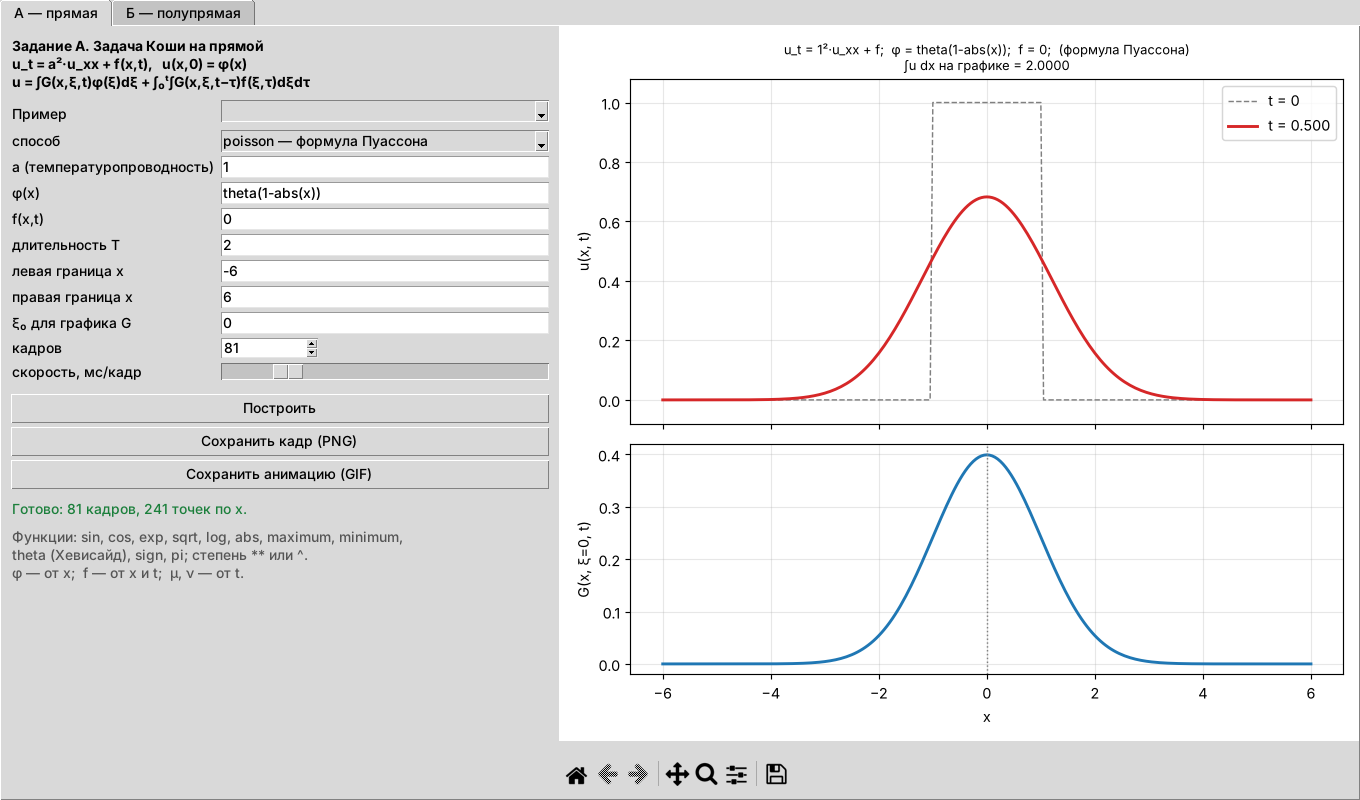
\includegraphics[width=\textwidth]{app_a.png}
\caption{Приложение, вкладка А: поля ввода и готовые примеры слева; сверху
решение в момент $t$ и начальное условие, внизу функция Грина $G(x,0,t)$;
ползунок и кнопка $\blacktriangleright$ под графиком~--- анимация}
\label{fig:appA}
\end{figure}

\subsection{Результаты и проверка}

На рис.~\ref{fig:aframes} слева~--- остывание прямоугольного импульса: углы
сглаживаются мгновенно (бесконечная скорость распространения тепла), максимум
убывает, площадь $\int u\,dx=2$ сохраняется (на графике программы она выводится
в заголовке). Справа~--- нагрев пульсирующим источником, посчитанный через функцию Грина.

\begin{figure}[H]
\centering
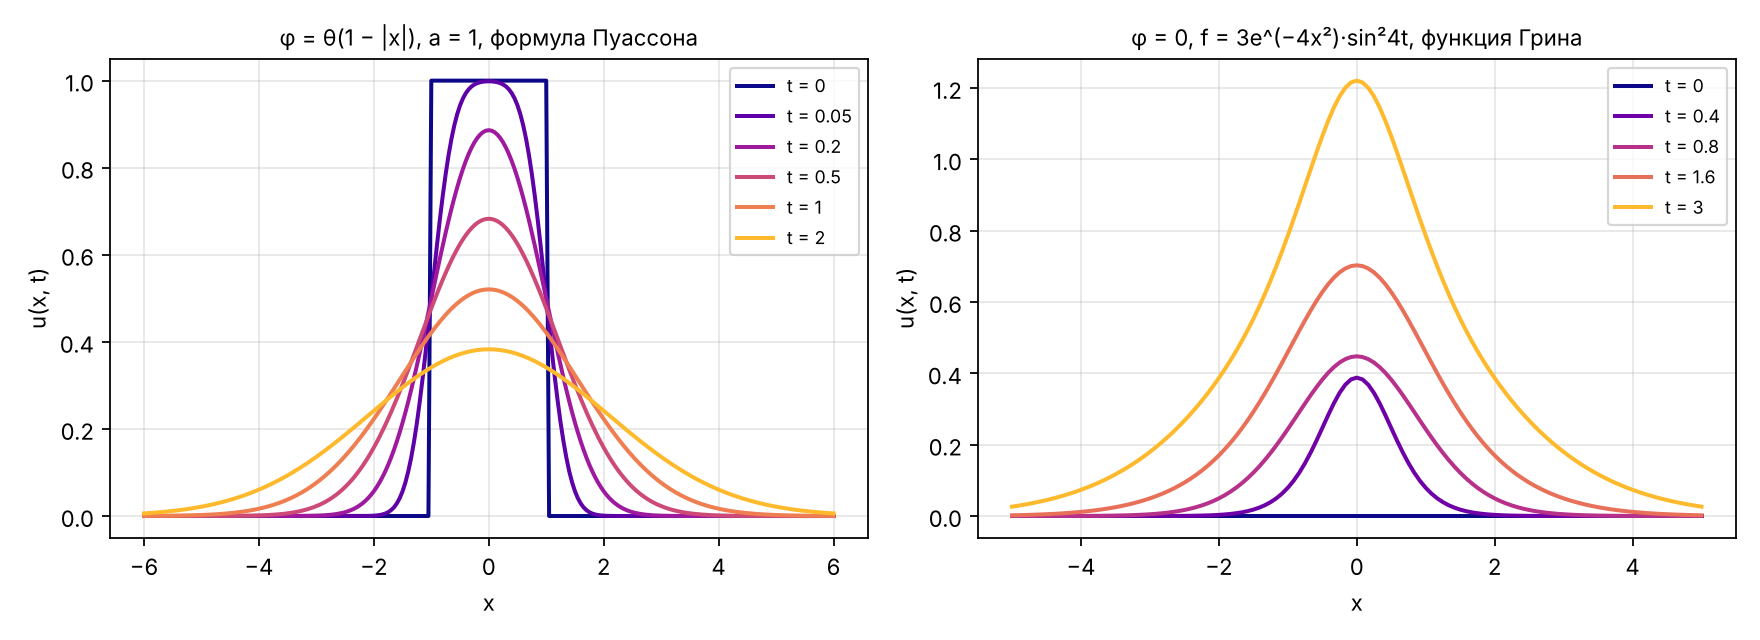
\includegraphics[width=\textwidth]{a_frames.png}
\caption{Задание А: решения в несколько моментов времени}
\label{fig:aframes}
\end{figure}

Сравнение с точными решениями (рис.~\ref{fig:acheck} и файл \code{tests/test\_line.py}):
\begin{itemize}
  \item $\varphi=e^{-x^2}$: $u=\dfrac{1}{\sqrt{1+4a^2t}}\exp\!\left(-\dfrac{x^2}{1+4a^2t}\right)$~--- ошибка $<10^{-9}$;
  \item $\varphi=\theta(x)$: $u=\tfrac12\bigl(1+\operatorname{erf}\frac{x}{2a\sqrt t}\bigr)$~---
        $<10^{-6}$ (Пуассон) и $3\cdot10^{-5}$ (Грин, разрыв в узле сетки);
  \item $\varphi=\sin kx$: $u=e^{-a^2k^2t}\sin kx$;\quad $\varphi=x^2$: $u=x^2+2a^2t$;
  \item $f=1$: $u=t$;\quad $\varphi=\sin2x$, $f=t$: $u=e^{-4a^2t}\sin2x+t^2/2$.
\end{itemize}

\begin{figure}[H]
\centering
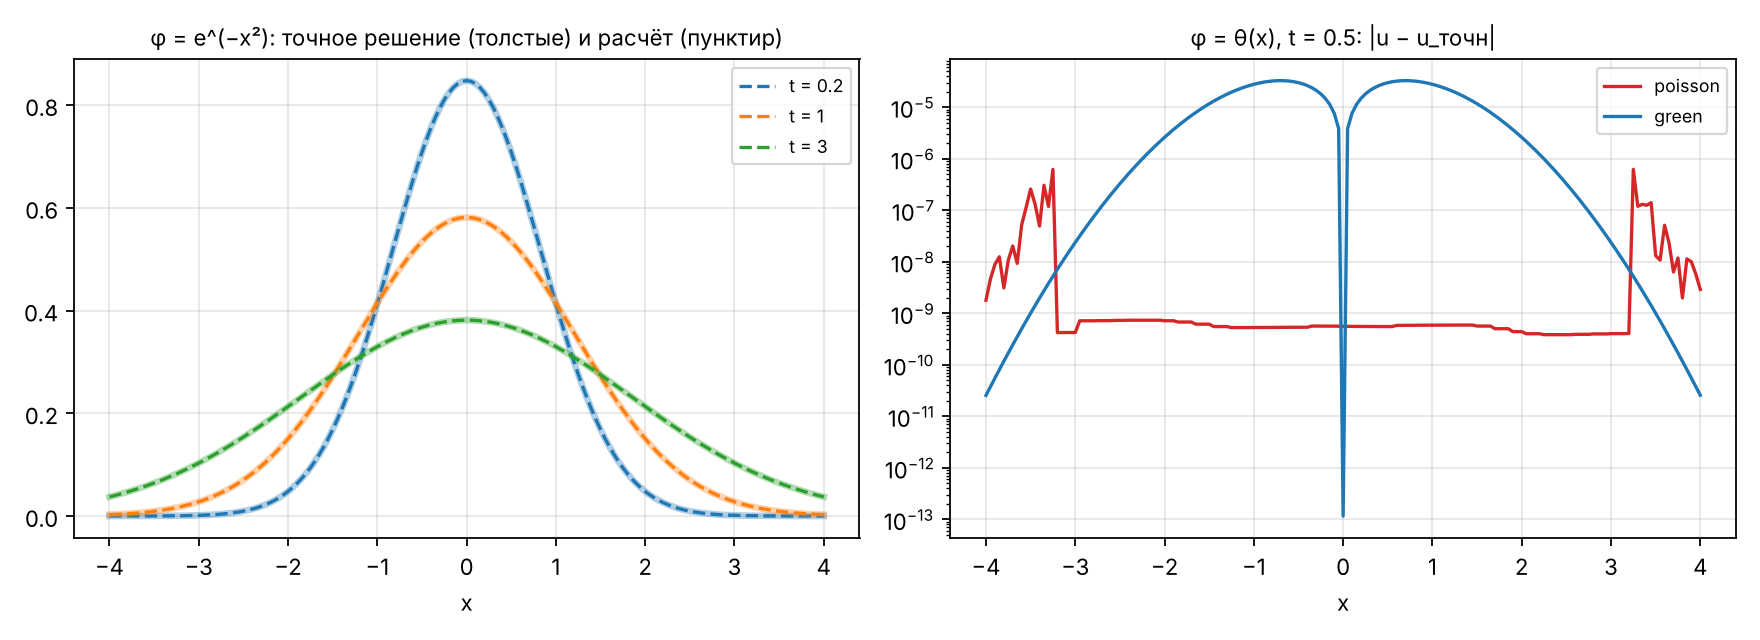
\includegraphics[width=\textwidth]{a_check.png}
\caption{Слева: расчёт совпадает с точным решением для $\varphi=e^{-x^2}$;
справа: ошибка обоих способов для ступеньки $\varphi=\theta(x)$}
\label{fig:acheck}
\end{figure}

% ======================================================================
\section{Задание Б. Полупрямая, функция Грина}

\subsection{Постановка задачи}

\begin{equation}\label{eq:B}
\begin{gathered}
  u_t=a^{2}u_{xx}+f(x,t),\qquad x>0,\ t>0;\qquad u(x,0)=\varphi(x),\ x\ge0;\\
  u_x(0,t)=\mu(t)\cdot\nu(t),\qquad t>0 .
\end{gathered}
\end{equation}
\textbf{Вариант группы}~--- граничное условие II рода (задан тепловой поток
через границу), правая часть~--- произведение двух вводимых функций $\mu(t)$ и $\nu(t)$.
Обозначим $g(t)=\mu(t)\nu(t)$. Если $g<0$, то $u$ убывает по $x$ у границы~---
тепло втекает в стержень; $g>0$~--- вытекает; $g=0$~--- изоляция.

\subsection{Метод}

Функция Грина для полупрямой с условием II рода строится методом отражений:
к источнику в точке $\xi$ добавляется такой же источник в точке $-\xi$.
Сумма чётна по $x$, поэтому $\partial_xG_2=0$ при $x=0$:
\begin{equation}\label{eq:G2}
  G_2(x,\xi,t)=G(x,\xi,t)+G(x,-\xi,t).
\end{equation}
По формуле Грина решение задачи~\eqref{eq:B}:
\begin{equation}\label{eq:solB}
\begin{split}
  u(x,t)={}&\int_{0}^{\infty}G_2(x,\xi,t)\varphi(\xi)\,d\xi
        -a^2\!\int_{0}^{t}G_2(x,0,t-\tau)\,\mu(\tau)\nu(\tau)\,d\tau\\
        &+\int_{0}^{t}\!d\tau\int_{0}^{\infty}G_2(x,\xi,t-\tau)f(\xi,\tau)\,d\xi .
\end{split}
\end{equation}
Здесь $G_2(x,0,s)=\dfrac{1}{a\sqrt{\pi s}}e^{-x^2/(4a^2s)}$ имеет
интегрируемую особенность $1/\sqrt{s}$ при $\tau\to t$. Замена
$t-\tau=\sigma^2$ её убирает:
\begin{equation}\label{eq:bnd}
  -a^2\!\int_{0}^{t}G_2(x,0,t-\tau)\,g(\tau)\,d\tau
  =-\frac{2a}{\sqrt\pi}\int_{0}^{\sqrt t}g\bigl(t-\sigma^2\bigr)\,
   \exp\!\left(-\frac{x^2}{4a^2\sigma^2}\right)d\sigma .
\end{equation}
Первый интеграл~\eqref{eq:solB} берётся по $\xi\in[\max(0,x-W),\,x+W]$,
$W=6\cdot2a\sqrt t$ (вне отрезка $G_2<10^{-16}$), и он, и~\eqref{eq:bnd}~---
адаптивной формулой Симпсона; источник~--- как в задании А.

Дополнительно (выбор «1» в программе) реализовано условие I рода
$u(0,t)=\mu(t)\nu(t)$: $G_1=G(x,\xi,t)-G(x,-\xi,t)$, граничное слагаемое
после замены $w=x/(2a\sqrt{t-\tau})$:
$\dfrac{2}{\sqrt\pi}\displaystyle\int_{x/(2a\sqrt t)}^{\infty}
 g\Bigl(t-\frac{x^2}{4a^2w^2}\Bigr)e^{-w^2}dw$.

\subsection{Программа}

Файл \code{heatlab/halfline.py}: класс \code{HeatHalfLine(a, phi, mu, nu, kind, f)},
методы \code{initial\_part}, \code{boundary\_part}, \code{source\_part} (три
слагаемых~\eqref{eq:solB}) и \code{u(x, t)}. Анимацию выводит \code{task\_b.py}
(файл \code{task\_b.gif}) и вкладка «Б» приложения (рис.~\ref{fig:appB}): решение,
функция Грина $G_2(x,\xi_0,t)$ и граничная функция $\mu\nu$ с отметкой текущего момента.

\begin{figure}[H]
\centering
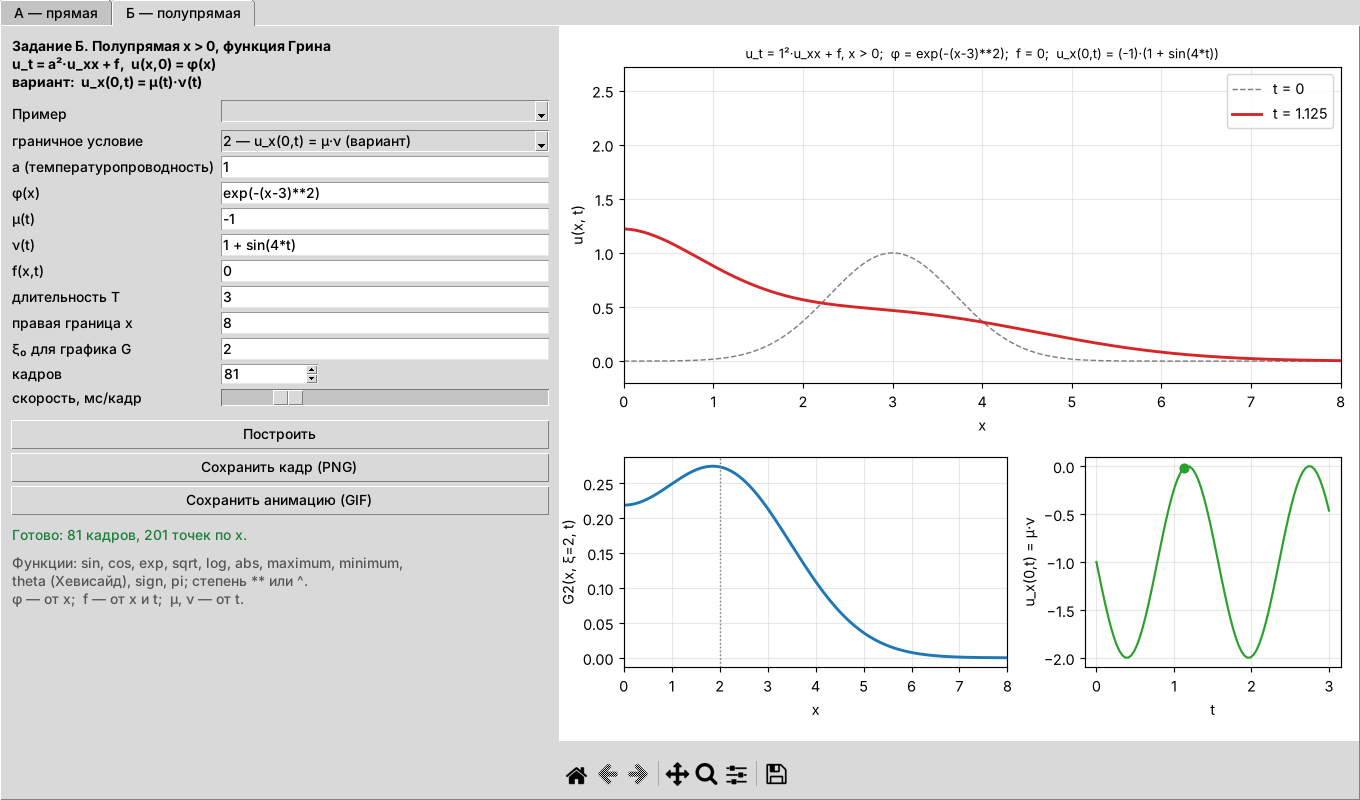
\includegraphics[width=\textwidth]{app_b.png}
\caption{Приложение, вкладка Б: $u_x(0,t)=(-1)\cdot(1+\sin4t)$, $\varphi=e^{-(x-3)^2}$}
\label{fig:appB}
\end{figure}

\subsection{Результаты и проверка}

\begin{figure}[H]
\centering
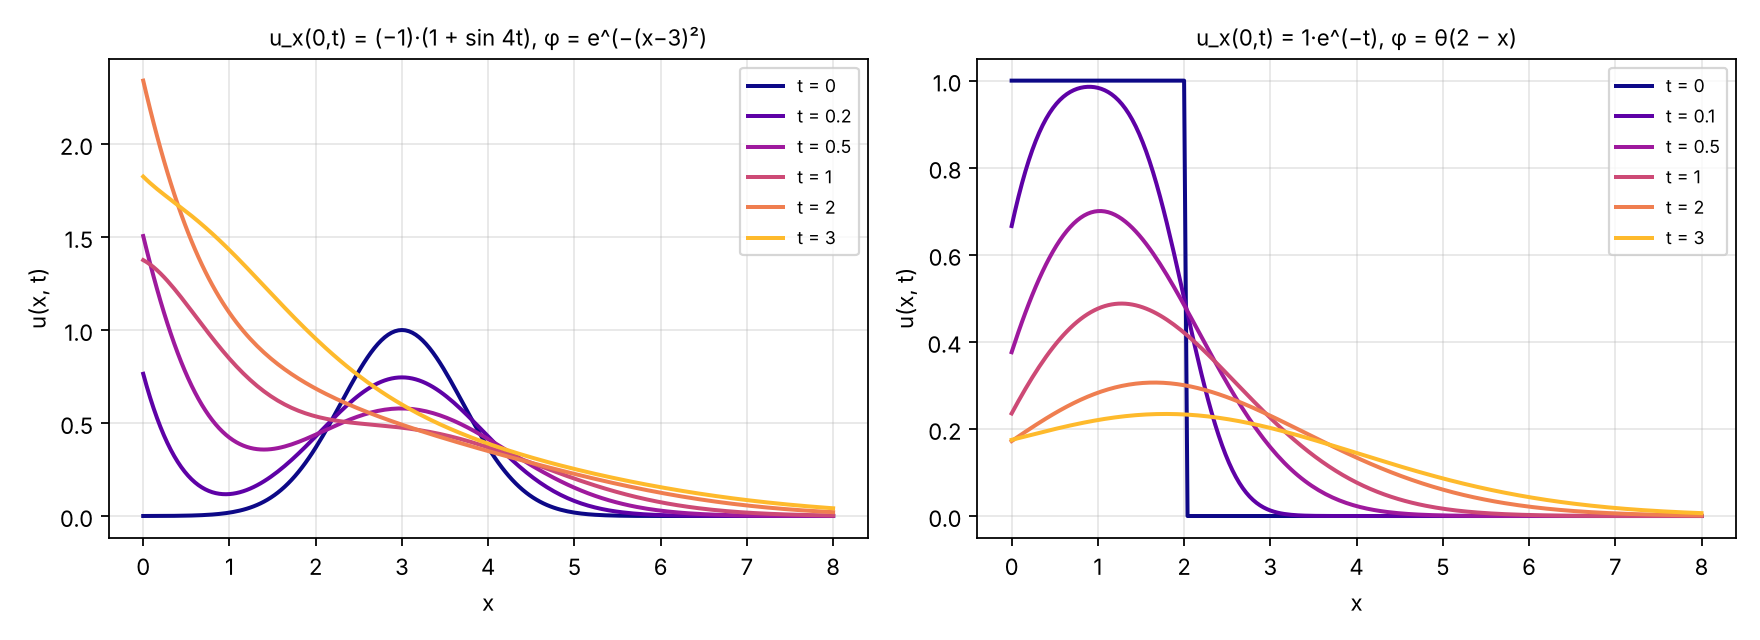
\includegraphics[width=\textwidth]{b_frames.png}
\caption{Задание Б. Слева: пульсирующий приток тепла через границу,
справа: отток $u_x(0,t)=e^{-t}$ из нагретого участка $[0,2]$}
\label{fig:bframes}
\end{figure}

Проверка (рис.~\ref{fig:bcheck}, файл \code{tests/test\_halfline.py}):
\begin{itemize}
  \item $\varphi=0$, $\mu\nu=-q$ (постоянный поток): точное решение
        $u=2q\Bigl[a\sqrt{t/\pi}\,e^{-z^2}-\frac{x}{2}\operatorname{erfc}z\Bigr]$,
        $z=\frac{x}{2a\sqrt t}$~--- ошибка $<10^{-9}$;
  \item переменный поток $\mu\nu=2t$~--- сравнение с интегралом Дюамеля по решению
        с единичным потоком;
  \item граничное условие: численная производная $u_x(0,t)$ совпадает с $\mu(t)\nu(t)$;
  \item $\varphi=\cos kx$, $\mu\nu=0$: $u=e^{-a^2k^2t}\cos kx$; при изоляции
        тепло $\int_0^\infty u\,dx$ сохраняется; $f=1$: $u=t$;
  \item I рода: $u(0,t)=1$ даёт $u=\operatorname{erfc}\frac{x}{2a\sqrt t}$.
\end{itemize}

\begin{figure}[H]
\centering
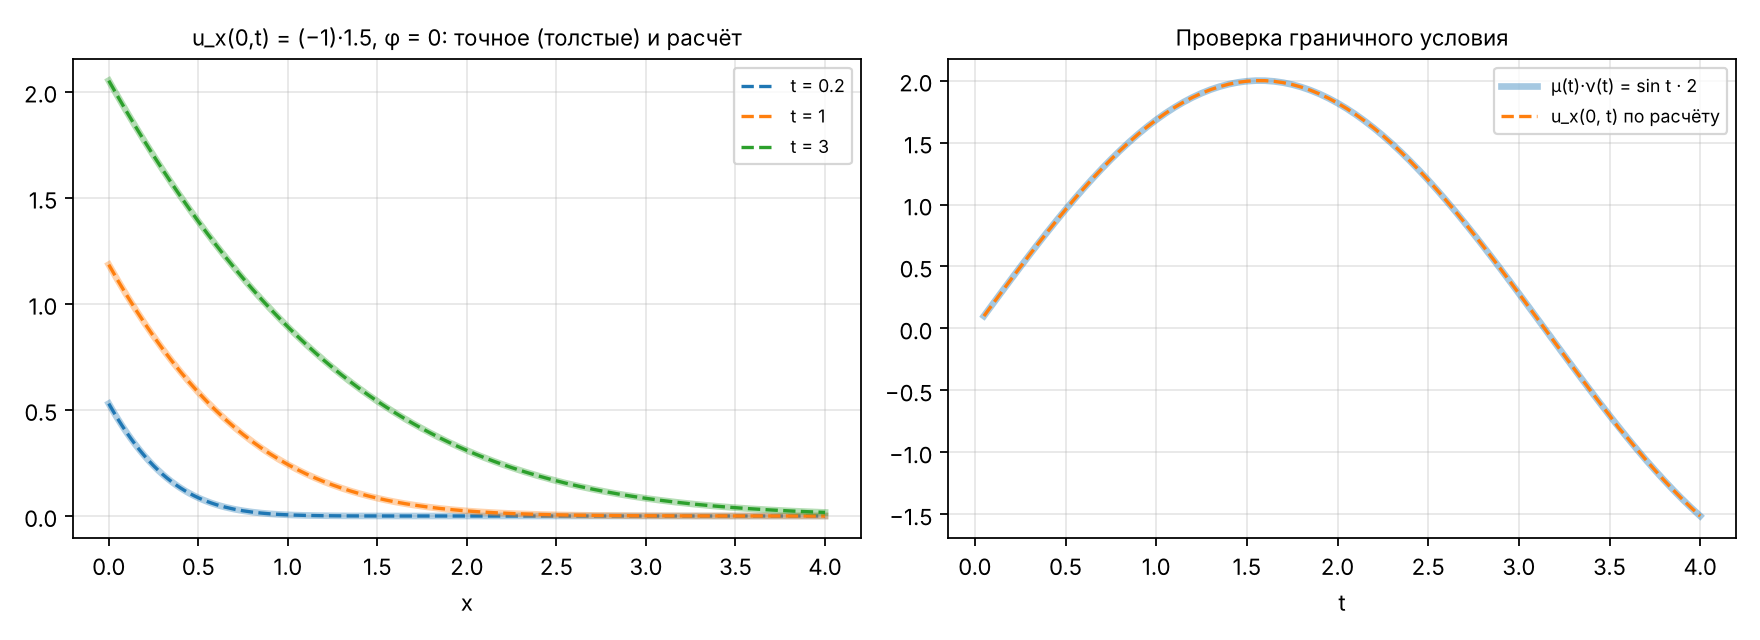
\includegraphics[width=\textwidth]{b_check.png}
\caption{Слева: постоянный поток, расчёт и точное решение;
справа: $u_x(0,t)$ по расчёту совпадает с заданным $\mu(t)\nu(t)=2\sin t$}
\label{fig:bcheck}
\end{figure}

% ======================================================================
\section{Запуск}

Из папки \code{lab3\_heat}: \code{python app.py}~--- приложение;
\code{python task\_a.py}, \code{python task\_b.py}~--- диалог или ключи
(\code{--phi}, \code{--mu}, \code{--nu}, \code{--method}, \code{--kind}, \code{--T}, \dots);
\code{python -m unittest discover -s tests -t .}~--- 23 теста. Функции вводятся
строкой: \code{exp(-(x-3)**2)}, \code{theta(1-abs(x))}, \code{1+sin(4*t)}.
Подробное объяснение всех формул и параметров с графиками~--- в файле
\code{report/explanation3.pdf}.

\end{document}
